% Images for Introductory Chemistry (c) by Dale J. Brugh

% Images for Introductory Chemistry is licensed under a
% Creative Commons Attribution-ShareAlike 4.0 International License.

% You should have received a copy of the license along with this 
% work. If not, see http://creativecommons.org/licenses/by-sa/4.0/.

\documentclass[tikz]{standalone}
\usepackage[T1]{fontenc}
\renewcommand{\rmdefault}{ptm}	% Sets roman font to Times
\usepackage[scaled=0.92]{helvet}
\usepackage[subscriptcorrection,slantedGreek,nofontinfo,mtpcal]{mtpro2}
\begin{document}
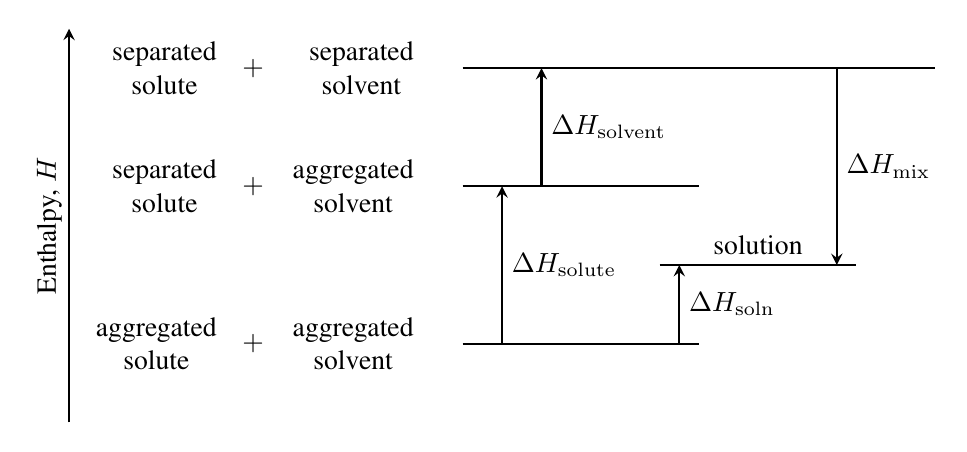
\begin{tikzpicture}[>=stealth, scale=1.0, every node/.style={scale=1.0}]
% Enthalpy Axis and Label
\draw [->,thick] (-5,-1) -- (-5,4);
\node [right,rotate=90] at (-5.25,0.5) {Enthalpy, $H$};
% Aggregated solute and aggregated solvent level
\draw [thick] (0,0) -- (3,0);
\node [align=center, left] at (-3,0) {aggregated \\ solute};
\node [left] at (-2.4,0) {$+$};
\node [align=center,left] at (-0.5,0) {aggregated \\ solvent};
% Aggregated solvent and separated solute
\draw [thick] (0,2) -- (3,2);
\draw [->,thick] (0.5,0) -- (0.5,2);
\node [right] at (0.5,1) {$\Delta H_{\mathrm{solute}}$};
\node [align=center, left] at (-3,2) {separated \\ solute};
\node [left] at (-2.4,2) {$+$};
\node [align=center,left] at (-0.5,2) {aggregated \\ solvent};
% Separated solvent and separated solute
\draw [thick] (0,3.5) -- (6,3.5);
\draw [->,thick] (1,2) -- (1,3.5);
\node [right] at (1,2.75) {$\Delta H_{\mathrm{solvent}}$};
\node [align=center, left] at (-3,3.5) {separated \\ solute};
\node [left] at (-2.4,3.5) {$+$};
\node [align=center,left] at (-0.5,3.5) {separated \\ solvent};
% Mixture
\draw [thick] (2.5,1) -- (5,1);
\node [above] at (3.75,1) {solution};
\draw [->,thick] (4.75,3.5) -- (4.75,1);
\node [right] at (4.75,2.25) {$\Delta H_{\mathrm{mix}}$};
% Solution Enthlapy
\draw [->,thick] (2.75,0) -- (2.75,1);
\node [right] at (2.75,0.5) {$\Delta H_{\mathrm{soln}}$};
\end{tikzpicture}
\end{document}